\begin{name}
	{\tenchude}
	{\tendethi}
	{\tentruong}
	{\thoigian}
\end{name}
\Opensolutionfile{ansbook}[ans/ansbookDe3]
\TN
\Opensolutionfile{ans}[ans/ansDe3-TN1]
\begin{ex}%[1D6N1-2]%[Dự án đề kiểm tra Toán 11 GHKII NH23-24 - Nguyễn Ngọc Dũng]%[De-3]
	Cho $a$ là số thực dương khác $1$. Giá trị của biểu thức $P=a^{\frac{2}{3}}\sqrt{a}$ bằng
	\choice
	{$a^3$}
	{$a^{\frac{2}{3}}$}
	{\True $a^{\frac{7}{6}}$}
	{$a^{\frac{5}{6}}$}
	\loigiai{Ta có $P=a^{\frac{2}{3}}\sqrt{a}=a^{\frac{2}{3}}a^{\frac{1}{2}}=a^{\frac{7}{6}}$.}
	\end{ex}

\begin{ex}%[1D6N2-2]%[Dự án đề kiểm tra Toán 11 GHKII NH23-24 - Nguyễn Ngọc Dũng]%[De-3]
Cho $a$ là một số thực dương khác $1$. Giá trị của biểu thức $\log_a{a^{\frac{1}{3}}}$ bằng
\choice
{$-\dfrac{1}{3}$}
{\True $\dfrac{1}{3}$}
{$3$}
{$-3$}
\loigiai{
Ta có $\log_a{a^{\frac{1}{3}}}=\dfrac{1}{3}\log_a{a}=\dfrac{1}{3}$.
}
\end{ex}

\begin{ex}%[1D6N3-3][Dự án 2025 - Đề cấu trúc mới của Bộ theo
	\immini[thm]
	{
	Đường cong trong hình vẽ là đồ thị của hàm số nào dưới đây?
	\choice
	{$y=\dfrac{x-1}{x}$}
	{$y=\sqrt{x-1}$}
	{$y=\ln x$}
	{\True $y=\log_2x$}
	}
	{
	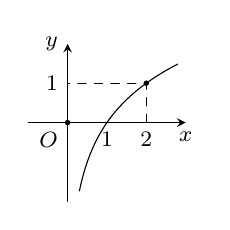
\begin{tikzpicture}[scale=.5, font=\footnotesize, line join=round, line cap=round, >=stealth]
	\draw[->](-1,0)--(3,0)node[below]{$x$};
	\draw[->](0,-2)--(0,2)node[left]{$y$};
	\draw[smooth, samples=100, domain=0.3:2.8]plot(\x,{(ln (\x))/(ln 2)});
	\draw[dashed]
	(2,0)--(2,1)--(0,1)
	;
	\draw
	(0,0)node[below left]{$O$}
	(1,0)node[below]{$1$}
	(0,1)node[left]{$1$}
	(2,0)node[below]{$2$};
	;
	\fill
	(0,0)circle(2pt)
	(2,1)circle(2pt)
	;
	\end{tikzpicture}
	}
	\loigiai
	{
	Đồ thị đã cho là đồ thị của hàm số logarit.\\
	Do đồ thị hàm số đi qua điểm $(2;1)$ nên đồ thị đã cho là của hàm số $y=\log_2x$.
	}
	\end{ex}

	\begin{ex}%[1H8N1-1]
		Trong các mệnh đề sau, mệnh đề nào đúng?
		\choice
		{\True Góc giữa hai đường thẳng $a$ và $b$ bằng góc giữa hai đường thẳng $a$ và $c$ khi $b$ song song hoặc trùng với đường thẳng $c$}
		{Góc giữa hai đường thẳng là góc nhọn}
		{Góc giữa hai đường thẳng $a$ và $b$ bằng góc giữa hai đường thẳng $a$ và $c$ thì $b$ song song với $c$}
		{Góc giữa hai đường thẳng bằng góc giữa hai véc-tơ chỉ phương của hai đường thẳng đó}
		\loigiai{
		Góc giữa hai đường thẳng $a$ và $b$ bằng góc giữa hai đường thẳng $a$ và $c$ khi $b$ song song hoặc trùng với đường thẳng $c$.
		}
		\end{ex}

		\begin{ex}%[1H8N3-1]%[Dự án đề kiểm tra Toán 11 GHKII NH23-24- Huỳnh Xuân Tín]%[THPT Hoàng Văn Thụ- Hà Nội]
			% \immini[thm]{	
				Cho hình lăng trụ đứng $ABC. A' B' C'$, có đáy $ABC$ là tam giác vuông tại $B$. Hình chiếu vuông góc của điểm $C$ trên $\left(ABB' A'\right)$ là điểm nào sau đây? \choice
			{$A'$}
			{$B'$}
			{$A$}
			{\True $B$}
			%}{
			% \begin{tikzpicture}[scale=.7,>=stealth, font=\footnotesize, line join=round, line cap=round]
			% \def\a{4}
			% \def\h{4.5}
			% \path 	(0:0) coordinate (A)
			% ++(0:\a) coordinate (C)
			% ++(-150:3*\a/4) coordinate (B)
			% ($(A)+(90:\h)$) coordinate (A')
			% ($(B)+(90:\h)$) coordinate (B')
			% ($(C)+(90:\h)$) coordinate (C');
			% \draw[dashed,thick] 	(A)--(C);
			% \draw[thick]	(C)--(C') 	(B)--(B')	(A)--(A') (A)--(B)--(C) (A')--(B')--(C')--cycle;
			% \foreach \x/\g in {A/180,B/-45,C/0,A'/180,B'/-45,C'/0}
			% \fill[black] 	(\x) circle (1pt)
			% ($(\g:4mm)+(\x)$) node {$\x$};
			% \draw pic[draw,angle radius=3mm]{right angle=C--B--A};
			% \end{tikzpicture}}
			
			\loigiai{Ta có $BC\perp AB$ (vì $\triangle ABC$ vuông tại $B$).\\
			$ABC. A' B' C'$ là lăng trụ đứng nên $A'A\perp BC$.\\
			$A'A$ và $AB$ cắt nhau trong $(ABB'A')$, suy ra $CB\perp (ABB'A')$.\\
			Vậy hình chiếu vuông góc của điểm $C$ trên $\left(ABB' A'\right)$ là điểm $B$.	}
			\end{ex}

\begin{ex}%[1H8N4-1]%[Dự án đề kiểm tra Toán 11 GHKI NH23-24-Võ Thị Thùy Trang]%[THPT MarieCurie- Tp HCM]
Chọn khẳng định đúng trong các khẳng định sau?
\choice
{Hình chóp có đáy là đa giác đều là hình chóp đều}
{Hình lăng trụ có đáy là một đa giác đều là hình lăng trụ đều}
{Hình lăng trụ tứ giác đều là hình lập phương}
{\True Hình chóp đều là hình chóp có đáy là đa giác đều và các cạnh bên bằng nhau}
\loigiai{
Theo lý thuyết ta có hình chóp đều là hình chóp có đáy là đa giác đều và các cạnh bên bằng nhau.
}
\end{ex}

\begin{ex}%[1H8N6-1]%[Dự án soạn đề kiểm tra Toán 11 HKII NH24-25- Mui Doan]%[CTST_1_OTHK2-De02]
Cho các mệnh đề sau
\begin{enumerate}[(I)]
\item Góc giữa đường thẳng và mặt phẳng bằng góc giữa đường thẳng đó và hình chiếu của nó trên mặt phẳng đã cho.
\item Góc giữa đường thẳng $a$ và mặt phẳng bằng góc giữa đường thẳng $b$ và mặt phẳng khi $a$ và $b$ cùng phương.
\item Góc giữa đường thẳng $a$ và mặt phẳng $(P)$ bằng góc giữa đường thẳng $a$ và mặt phẳng  $(Q)$ thì $(P) \parallel (Q)$.
\item Góc giữa đường thẳng $a$ và mặt phẳng $(P)$ bằng góc giữa đường thẳng $b$ và mặt phẳng  $(P)$ thì $a$ song song với $b$.
\end{enumerate}
Có bao nhiêu mệnh đề đúng trong các mệnh đề trên?
\choice
{$1$}
{\True$2$}
{$3$}
{$4$}
\loigiai{
\begin{enumerate}[(I)]
\item Góc giữa đường thẳng và mặt phẳng bằng góc giữa đường thẳng đó và hình chiếu của nó trên mặt phẳng đã cho $\longrightarrow$ đúng.
\item Góc giữa đường thẳng $a$ và mặt phẳng bằng góc giữa đường thẳng $b$ và mặt phẳng khi $a$ và $b$ cùng phương $\longrightarrow$ đúng.
\item Góc giữa đường thẳng $a$ và mặt phẳng $(P)$ bằng góc giữa đường thẳng $a$ và mặt phẳng  $(Q)$ thì $(P) \parallel (Q)$ $\longrightarrow$ sai vì $(P)$ có thể không song song với $(Q)$.
\item Góc giữa đường thẳng $a$ và mặt phẳng $(P)$ bằng góc giữa đường thẳng $b$ và mặt phẳng  $(P)$ thì $a$ song song với $b$ $\longrightarrow$ sai vì $a$ có thể không song song với $b$.
\end{enumerate}
}
\end{ex}

\begin{ex}%[1H8N7-1]%[Dự án đề kiểm tra Toán 11 HKII NH23-24-  Pham Quoc Toan]%[THPT TRUNGHOCTHUCHANH- Tp HCM]
Cho khối lăng trụ có diện tích đáy $B$ và chiều cao $h$. Thể tích $V$ của khối lăng trụ đã cho được tính theo công thức nào dưới đây?
\choice
{$V = 6 Bh$}
{$V = \dfrac{4}{3} B h$}
{$V = \dfrac{1}{3} B h$}
{\True $V = B h$}
\loigiai{
Thể tích $V$ của khối lăng trụ đã cho được tính bởi $V = B h$.
}
\end{ex}

\begin{ex}%[1D9N1-1]%[Dự án đề kiểm tra Toán 11 GHKI NH23-24- Tổng Nguyễn]%[THPT Phạm Phú Thứ - Đà Nẵng]
Cho $A$ và $B$ là hai biến cố. Biến cố: \lq\lq Cả $A$ và $B$ đều xảy ra\rq\rq  \ là biến cố nào sau đây?
\choice
{\True $AB$}
{$A \cup B$}
{$A\cup \overline{B}$}
{$A \overline{B}$}
\loigiai{ Biến cố: \lq\lq Cả $A$ và $B$ đều xảy ra\rq\rq  \ là biến cố $AB$.
}
\end{ex}
\begin{ex}%[1D9N2-3]%[Dự án đề kiểm tra Toán 11 GKII NH23-24- Lê Hữu Kiệt]%[THPT Trần Khải Nguyên -- Hồ Chí Minh]
	Cho $A$, $B$ là hai biến cố xung khắc. Biết ${\rm P}(A)=\dfrac{1}{3}$, ${\rm P}(B)=\dfrac{1}{4}$. Tính ${\rm P}(A \cup B)$.
	\choice
	{$\dfrac{1}{12}$}
	{$\dfrac{1}{7}$}
	{\True $\dfrac{7}{12}$}
	{$\dfrac{1}{2}$}
	\loigiai{
	Ta có $A$ và $B$ là hai biến cố xung khắc nên\\
	\centerline{${\rm P}(A \cup B) ={\rm P}(A)+{\rm P}(B)=\dfrac{1}{3}+\dfrac{1}{4} = \dfrac{7}{12}$.}
	}
	\end{ex}

\begin{ex}%[1D7N1-1]ID%[Dự án đề kiểm tra Toán 11 GHKI NH23-24- Phan Trung Hiếu]%[THPT Nguyễn Hữu Huân- Tp HCM]
Cho hàm số $y = f(x)$ có đạo hàm tại điểm $x_0$. Chọn phát biểu đúng.
\choice
{\True $f^\prime(x_0) = \lim\limits_{x \to x_0} \dfrac{f(x) - f(x_0)}{x - x_0}$}
{$f^\prime(x_0) = \lim\limits_{x \to x_0} \dfrac{f(x) + f(x_0)}{x - x_0}$}
{$f^\prime(x_0) = \lim\limits_{x \to x_0} \dfrac{f(x) - f(x_0)}{x + x_0}$}
{$f^\prime(x_0) = \lim\limits_{x \to x_0} \dfrac{f(x) + f(x_0)}{x + x_0}$}
\loigiai{
Phát biểu đúng là $f^\prime(x_0) = \lim\limits_{x \to x_0} \dfrac{f(x) - f(x_0)}{x - x_0}$.
}
\end{ex}

\begin{ex}%[1D7N1-4]
	Một chuyển động thẳng xác định bởi phương trình $s=t^3 -3t^2 +5t+2$, trong đó $t$ tính bằng giây và $s$ tính bằng mét. Vận tốc của chuyển động khi $t=3$ là
	\choice
	{\True $14 ~\mathrm{m} / \mathrm{s}$}
	{$15 ~\mathrm{m} / \mathrm{s}$}
	{$17 ~\mathrm{m} / \mathrm{s}$}
	{$12 ~\mathrm{m} / \mathrm{s}$}
	\loigiai{
	Ta có vận tốc tức thời có phương trình là $v=s'(t)=3t^2-6t+5$.\\
	Do đó vận tốc của chuyển động ứng với $t=3$ là $v(3)=14 ~\mathrm{m} / \mathrm{s}$.
	}
	\end{ex}
\Closesolutionfile{ans}

\TNTF
\Opensolutionfile{ans}[ans/ansDe3-TN2]
\begin{ex}%[1D7H1-1]%[1D7H2-1]%[1D7H2-2]%[tex hóa đề ck2 - form 2025 - đợt 2 - GV Thái Bảo]
	Một chuyển động thẳng có quãng đường di chuyển được xác định bởi phương trình $s(t)=2t^2+t-1$, trong đó $s$ tính bằng mét và $t$ tính bằng giây.
	\choiceTF{\True Tốc độ tức thời của chuyển động tại thời điểm $t_0$ là $v(t_0)=\lim\limits_{t\to t_0} \dfrac{s(t)-s(t_0)}{t-t_0}$}
	{Tại thời điểm $t=2$ tốc độ tức thời của chuyển động là $10$ m/s}
	{$s(3)-s'(1)=3$}
	{\True Phương trình $s(t)-\left[\left(t+1\right).s(t)\right]'+27=0$ có $2$ nghiệm trái dấu}
	\loigiai{
	\begin{itemchoice}
	\itemch Tốc độ tức thời của chuyển động tại thời điểm $t_0$ là $v'(t_0)=\lim\limits_{t\to t_0} \dfrac{s(t)-s(t_0)}{t-t_0}$.
	\itemch Tốc độ tức thời tại thời điểm $t=2$ là \[\lim\limits_{t\to 2} \dfrac{s(t)-s(2)}{t-2}=\lim\limits_{t\to 2} \dfrac{2t^2+t-1-9}{t-2}=\lim\limits_{t\to 2} \dfrac{\left(t-2\right)\cdot\left(2t+5\right)}{t-2}=\lim\limits_{t\to 2} \left(2t+5\right)=9.\]
	\itemch Ta có $s(3)=2\cdot3^2+3-1=20$ suy ra $s'(t)=4t+1\Rightarrow s'(1)=5$
	\itemch Ta có
	\begin{eqnarray*}
	&	&\left[\left(t+1\right)\cdot s(t)\right]^{{'}}\\
	&=	&\left(t+1\right)^{{'}} s(t)+\left(t+1\right)s'(t)\\
	&=	&1\cdot \left(2t^2+t-1\right)+\left(t+1\right)\left(4t+1\right)\\
	&=	&2t^2+t-1+4t^2+5t+1=6t^2+6t
	\end{eqnarray*}
	Xét phương trình
	\begin{eqnarray*}
	&	&s(t)-\left[\left(t+1\right)\cdot s(t)\right]^{{'}} 27=0\\
	&\Leftrightarrow	& 2t^2+t-1-\left(6t^2+6t\right)+27=0\\
	&\Leftrightarrow	&-4t^2-5t+26=0\\
	&\Leftrightarrow	& \hoac{	&{t=2} \\
	&{t=\dfrac{-13}{4}}.}
	\end{eqnarray*}
	Vậy phương trình đã cho có $2$ nghiệm trái dấu.
	\end{itemchoice}
	}
	\end{ex}

	\begin{ex}%[1D7H2-1]%[2025-TLDT11-Tăng Xuân Phú]
		Cho hàm số $f(x)=\dfrac{x-3}{x+2}$ và $g(x)=x\ln x$. Khi đó
		\choiceTF
		{\True Hàm số $f(x)$ có đạo hàm là $f'(x)=\dfrac{5}{\left(x+2\right)^2}$}
		{\True Hàm số $g(x)$ có đạo hàm là $g'(x)=\ln x+1$}
		{$f'\left(-1\right)-g'(\mathrm{e})=2$}
		{Phương trình $\left(x+2\right)^2f'(x)=g'(x)$ có hai nghiệm}
		\loigiai{
		\begin{itemchoice}
		\itemch Ta có\\ $f'(x)=\left(\dfrac{x-3}{x+2} \right)^{{'}}=\dfrac{\left(x-3\right)^{{'}}\cdot \left(x+2\right)-\left(x-3\right)\cdot \left(x+2\right)^{{'}}}{\left(x+2\right)^2}=\dfrac{x+2-x+3}{\left(x+2\right)^2}=\dfrac{5}{\left(x+2\right)^2}$.
		\itemch Ta có $g'(x)=\left(x\ln x\right)^{{'}}=x'\ln x+x\cdot \left(\ln x\right)^{{'}}=\ln x+1$.
		\itemch $\heva{&f'\left(-1\right)=\dfrac{5}{\left(-1+2\right)^2}=5\\&g'(\mathrm{e})=\ln \mathrm{e}+1=2} \Rightarrow f'\left(-1\right)\ne g'(\mathrm{e})$.
		\itemch Ta có
		\begin{align*}
		&\left(x+2\right)^2f'(x)=g'(x)\\
		\Leftrightarrow& \left(x+2\right)^2\cdot \dfrac{5}{\left(x+2\right)^2}=\ln x+1\\
		\Leftrightarrow& 5=\ln x+1\Leftrightarrow \ln x=4\\
		\Leftrightarrow& x=\mathrm{e}^4.
		\end{align*}
		\end{itemchoice}
		}
		\end{ex}
\Closesolutionfile{ans}

\TNSA
\Opensolutionfile{ans}[ans/ansDe3-TN3]
\begin{ex}%[10-11-EX-GK2-2425]%[Trần Tony]%[1D6H4-3]
Bất phương trình $\log_2(3x-20) \leq 7$ có bao nhiêu nghiệm nguyên trong khoảng $(-20; 36)$?
\shortans{29}
\loigiai{
Ta có $\log_2(3x-20) \leq 7\Leftrightarrow 0<3x-20\leq 2^7\Leftrightarrow \dfrac{20}{3}<x\leq \dfrac{148}{3}$.\\
Kết hợp với $x$ nguyên thuộc khoảng $(-20; 36)$, ta được $x\in\{7;8;\ldots 35\}$.\\
Vậy bất phương trình có $29$ nghiệm nguyên thỏa mãn.
}
\end{ex}

\begin{ex}%[1H8H5-4]
	Cho hình hộp chữ nhật $MNPQ.M'N'P'Q'$ có $MN=2$, $MQ=3$, $MM'=4$. Khoảng cách giữa hai đường thẳng $NP$ và $M'N'$ bằng bao nhiêu?
	\shortans{$4$}
	\loigiai{
	\immini{
	Ta có $\heva{&NP\perp NN'\\&M'N'\perp NN'.}$\\
	Do đó $NN'$ là đoạn vuông góc chung của $NP$ và $M'N'$.\\
	Vậy $\mathrm{d}(NP,M'N')=NN'=MM'=4$.
	}{
	\begin{tikzpicture}[scale=1, font=\footnotesize, line join=round, line cap=round, >=stealth]
	\path
	(0,0) coordinate (M)
	(-1,-1) coordinate (N)
	(3,0) coordinate (Q)
	($(N)+(Q)-(M)$) coordinate (P)
	($(M)+(0,2.5)$) coordinate (M')
	($(M')-(M)+(N)$) coordinate (N')
	($(M')-(M)+(P)$) coordinate (P')
	($(M')-(M)+(Q)$) coordinate (Q')
	(intersection of M--P and N--Q) coordinate (O)
	;
	\draw (M')--(N')--(P')--(Q')--(M') (N)--(N') (P)--(P') (Q)--(Q') (N)--(P)--(Q);
	\draw[dashed] (M')--(M)--(N) (M)--(Q);
	\foreach \x/\g in {M/180,N/-90,P/-90,Q/0,M'/90,N'/180,P'/90,Q'/0} \draw[fill=black] (\x) circle(1pt)++(\g:0.3)node{$\x$};
	\end{tikzpicture}
	}
	}
	\end{ex}

\begin{ex}%[1D9V2-4]%[Dự án - 2025_TLDT Toán 11]%[Nguyễn Tiến Liên]
Tại một trường trung học phổ thông $X$, có $12\%$ học sinh học giỏi môn Tiếng Anh, $35\%$ học sinh học giỏi môn Toán và $8\%$ học sinh học giỏi cả hai môn Toán, Tiếng Anh. Chọn ngẫu nhiên một học sinh từ trường $X$, tính xác suất để chọn được một học sinh không giỏi môn nào trong hai môn Toán, Tiếng Anh.
\shortans{$0{,}61$}
\loigiai{
Gọi $A$ là biến cố: \lq\lq Chọn được một học sinh giỏi môn Tiếng Anh\rq\rq, $B$ là biến cố: \lq\lq Chọn được một học sinh giỏi môn Toán\rq\rq.\\
Xác suất để chọn được một học sinh giỏi Toán hoặc giỏi Anh là\\
$\mathrm{P}(A\cup B)=\mathrm{P}(A)+\mathrm{P}(B)-\mathrm{P}(AB)=\dfrac{12}{100}+\dfrac{35}{100}-\dfrac{8}{100}=0{,}39$.\\
Xác suất để chọn được một em học sinh không giỏi môn nào trong hai môn Toán, Tiếng Anh là $\mathrm{P}(\overline{A\cup B})=1-\mathrm{P}(A\cup B)=1-0{,}39=0{,}61$.}
\end{ex}

\begin{ex}%[1D7C2-8]
	Một con lắc lò xo dao động điều hoà theo phương ngang trên mặt phẳng không ma sát, có phương trình chuyển động $x=4\cos \left(\pi t-\dfrac{2\pi}{3} \right)+4$ (cm), trong đó $t$ là thời gian tính bằng giây. Tìm thời điểm mà vận tốc tức thời của con lắc bằng $0$ (cm/s) là $t=\dfrac{a}{b}+k(k\in \mathbb{Z})$ (s), trong đó $a,b$ là các số nguyên và phân số $\dfrac{a}{b}$ là phân số tối giản. Tính tổng $a+b$?
	\shortans{$5$}
	\loigiai{
	Ta có $v(t)=x'=-4\pi \sin \left(\pi t-\dfrac{2\pi}{3} \right)$.\\
	Thời điểm mà vận tốc tức thời của con lắc bằng $0$ nghĩa là $v(t)=0$.
	\begin{eqnarray*}
	&\Leftrightarrow& -4\pi \sin \left(\pi t-\dfrac{2\pi}{3} \right)=0\\
	&\Leftrightarrow& \sin \left(\pi t-\dfrac{2\pi}{3} \right)=0\\
	&\Leftrightarrow& \pi t-\dfrac{2\pi}{3}=k\pi\\
	&\Leftrightarrow& t=\dfrac{2}{3}+k,\,\left(k\in\mathbb{Z}\right).
	\end{eqnarray*}
	Vậy các thời điểm mà vận tốc tức thời của con lắc bằng $0$ là $t=\dfrac{2}{3}+k(k\in \mathbb{Z})(s)$.\\
	Suy ra $a=2, b=3$, nên $a+b=5$.
	}
	\end{ex}
\Closesolutionfile{ans}

\TL
\begin{ex}%[$1{,}0$ điểm]%[1D7V2-1]%[Dự án đề kiểm tra Toán khối 11 HK2 NH23-24 - Dot 16 - Xuan Vy Pham]%[Trung học Thực hành - TP.HCM]
	Tính đạo hàm của các hàm số sau:
	\begin{enumerate}
	\begin{multicols}{2}
	\item $y=(x^3-3x+1)^{10}$.
	\item $y=\sqrt{\cot (x^2+3)}$.
	\end{multicols}
	\end{enumerate}
	\loigiai{Ta có
	\begin{enumerate}
	\item Ta có \begin{align*}
	y'&= \left[(x^3-3x+1)^{10}\right]'\\
	&=10(x^3-3x+1)^9(x^3-3x+1)'\\
	&=10(x^3-3x+1)^9(3x^2-3).
	\end{align*}
	\item Ta có \begin{align*}
	y'&= \left[\sqrt{\cot (x^2+3)}\right]'\\
	&=\dfrac{\left[\cot(x^2+3)\right]'}{2\sqrt{\cot (x^2+3)}}\\
	&=\dfrac{-1}{2\sin^2(x^2+3)\sqrt{\cot (x^2+3)}} \cdot (x^2+3)'\\
	&=\dfrac{-x}{\sin^2(x^2+3)\sqrt{\cot (x^2+3)}}.
	\end{align*}
	\end{enumerate}}
	\end{ex}

\begin{ex}%[Tex hóa Dự án Toán từ tâm K11 Đợt 3,Nhật Thiện]%[1H8V5-4]
Cho hình chóp $S.ABC$ có đáy là tam giác đều cạnh $a$. Hình chiếu vuông góc của $S$ trên $\left( ABC \right)$ là điểm $H$ thuộc cạnh $AB$ sao cho $HA=2HB$. Góc giữa đường thẳng $SC$ và $\left( ABC \right)$ bằng $60^\circ$. Tính khoảng cách giữa $SA$và $BC$ theo $a$.
\loigiai{
\immini{Áp dụng định lí cô-sin trong $\Delta AHC$ ta có
\begin{eqnarray*}
CH^2&=&CA^2+AH^2-2\cdot  CA\cdot  AH\cdot  \cos \widehat{CAH}\\
&=&a^2+\dfrac{4a^2}{9}+2\cdot  a\cdot  \dfrac{2a}{3}. \cos 60^\circ\\
&=&\dfrac{7a^2}{9}.
\end{eqnarray*}
Suy ra $CH=\dfrac{a\sqrt{7}}{3}$. \\
Ta có $HC$ là hình chiếu vuông góc của $SC$ trên $(ABC)$.\\
Nên $\left(SC; (ABC)\right)=\widehat{SCH}=60^\circ$. \\
Trong $\Delta SCH$, ta có \[SH=CH\cdot  \tan 60^\circ=\dfrac{a\sqrt{7}}{3}\cdot  \sqrt{3}=\dfrac{a\sqrt{21}}{3}.\]
Từ $A$ kẻ $Ax\parallel BC\Rightarrow BC\parallel (SAx)$.\\
Khi đó $\mathrm{d}(BC, SA)=\mathrm{d}\left(BC, (SAx)\right)=\mathrm{d}\left(B, (SAx)\right)$.}{
\begin{tikzpicture}[scale=1, font=\footnotesize, line join=round, line cap=round, >=stealth]
\path
(0,0) coordinate (B)
(3.5,-1.5) coordinate (A)
(4,0) coordinate (C)
($(B)!.3!(A)$) coordinate (H)
(H)+(0,3) coordinate (S)
(A)+(0:1) coordinate (m)
(A)+(180:3) coordinate (x) node[below]{$x$}
($(x)!.4!(A)$) coordinate (I)
($(S)!.5!(I)$) coordinate (K)
;
\draw (S)--(B)--(H)--(I)--(A)--(C)--cycle (S)--(H) (S)--(I) (H)--(K) (S)--(A);
\draw[dashed] (B)--(C) (H)--(C) (H)--(A);
\draw (A)--++(180:3.3) (A)--++(0:1.2);
\foreach \x/\dinh/\y in {S/H/B,H/K/I,H/I/A} \draw[fill = gray!50] ($(\dinh)!3pt!(\x)$)--($(\dinh)!3pt!(\x)+(\dinh)!3pt!(\y)-(\dinh)$)--($(\dinh)!3pt!(\y)$)--(\dinh)--cycle;
\foreach \p/\r in {B/180,A/-90,I/-90,C/0,S/90,H/-120,K/40}
\fill (\p) circle (1pt) node[shift={(\r:3mm)}]{$\p$};
\end{tikzpicture}
}
\noindent
Dựng $HI\perp Ax$ tại $I$. \\
Gọi $K$ là hình chiếu vuông góc của $H$trên $SI$. \\
Vì $\heva{
& Ax\perp HI \\
& Ax\perp SH }$ nên $Ax\perp (SHI)\Rightarrow (SAx)\perp (SHI)=SI$. \\
Mà $HK\perp SI\Rightarrow HK\perp (SAx)$. Vậy $\mathrm{d}\left(H, (SAx)\right)=HK$. \\
Trong $\Delta AIH$, ta tính được $HI=HA\cdot  \cos 60^\circ=\dfrac{2a}{3}\cdot  \dfrac{\sqrt{3}}{2}=\dfrac{a\sqrt{3}}{3}$. \\
Trong $\Delta SIH$, ta có $\dfrac{1}{HK^2}=\dfrac{1}{HS^2}+\dfrac{1}{HI^2}=\dfrac{9}{21a^2}+\dfrac{9}{3a^2}=\dfrac{24a^2}{7}\Rightarrow HK=\dfrac{a\sqrt{7}}{\sqrt{24}}$. \\
Vì $BH\cap (SAx)=A$ nên $\dfrac{\mathrm{d}\left(B, (SAx)\right)}{\mathrm{d}\left(H, (SAx)\right)}=\dfrac{BA}{HA}=\dfrac{3}{2}$. \\
Vậy $\mathrm{d}(BC, SA)=\mathrm{d}\left(B, (SAx)\right)=\dfrac{3}{2}\mathrm{d}\left(H, (SAx)\right)=\dfrac{3}{2}HK=\dfrac{a\sqrt{42}}{8}$.

}
\end{ex}
\begin{ex}%[1D9C1-3]%[tex hóa đề ck2 - form 2025 - đợt 2 - Ngô Tất Thành]
	Ba cầu thủ sút luân lưu $11$ m, mỗi người đá một lần với xác suất làm bàn tương ứng là $x$, $y$ và $0{,}6$ (với $ x > y$). Biết xác suất để ít nhất một trong ba cầu thủ ghi bàn là $97{,}6\% $ và xác suất để cả ba cầu thủ đều ghi ban là $ 33{,}6\% $. Tính xác suất để có đúng hai cầu thủ ghi bàn.
	% \shortans[0]{$0{,}452$}
	\loigiai{
	Gọi $A_i$ là biến cố \lq\lq người thứ $ i$ ghi bàn \lq\lq với $i=1,2,3$.\\
	Ta có các $A_i$ độc lập với nhau và $\mathrm{P}(A_1)=x$, $\mathrm{P}(A_2)=y$, $\mathrm{P}(A_3)=0{,}6$.\\
	Gọi A là biến cố \lq\lq Có ít nhất một trong ba cầu thủ ghi bàn \lq\lq\\
	B $\colon$ \lq\lq Cả ba cầu thủ đều ghi bàn\lq\lq\\
	C $\colon$ \lq\lq Có đúng hai cầu thủ ghi bàn\lq\lq\\
	Ta có $\overline A=\overline{A_1} \cdot \overline{A_2} \cdot \overline{A_3}\Rightarrow P\left(\overline A\right)=P\left(\overline{A_1}\right) \cdot P\left(\overline{A_2}\right) \cdot P\left(\overline{A_3}\right)=0Ơ,4(1-x)(1-y)$\\
	Nên $ P(A)=1-P\left(\overline A\right)=1-0{,}4(1-x)(1-y)=97{,}6\%=0{,}976$.\\
	Suy ra $(1-x)(1-y)=\dfrac{3}{50}\Leftrightarrow xy-x-y=-\dfrac{47}{50}$ $(1)$.\\
	Tương tự $ B=A_1 \cdot A_2 \cdot A_3$, suy ra\\
	$P(B)=P(A_1) \cdot P(A_2) \cdot P(A_3)=0{,}6xy=33{,}6\%=0{,}336$ hay là $ xy=\dfrac{14}{25} \qquad(2)$.\\
	Từ $(1)$ và $(2)$ ta có hệ $ \heva{
	&xy=\dfrac{14}{25}\\
	&x+y=\dfrac{3}{2}}$, \\
	giải hệ này kết hợp với $x > y$ ta tìm được\\
	$ x=0{,}8$ và $ y=0{,}7$.\\
	Ta có $C=\overline{A_1}{A_2}{A_3}+A_1\overline{A_2}{A_3}+A_1A_2\overline{A_3}$\\
	Nên $ P(C)=(1-x)y \cdot 0{,}6+x(1-y) \cdot 0{,}6+xy \cdot 0{,}4=0{,}452$.
	}
	\end{ex}
\Closesolutionfile{ansbook}
% \HetDe
% \label{De3}
% %
% \cleardoublepage
% \setcounter{page}{1}
% \rfoot{Trang \thepage/\pageref{DA3} - Đáp án trắc nghiệm Đề 3}
% \begin{center}
% 	\bfseries ĐÁP ÁN TRẮC NGHIỆM ĐỀ 3
% \end{center}

% \inputansbox{10}{ans/ansDe3-TN1}
% \inputansbox[3]{2}{ans/ansDe3-TN2}
% \inputansbox{3}{ans/ansDe3-TN3}
% \label{DA3}
%
